Quadcopter control is a complex, yet interesting problem. One of the reasons why this control problem is challenging is the fact that a quadcopter has six degrees of freedom, but only four inputs, which affects the linearity of the dynamics and makes the quadcopter under-actuated. 

In this chapter, we will take a look at the kinematics' and dynamics' equations that describe our quadcopter system for which we have drawn the block diagram shown in Figure \ref{dk}.

\begin{figure}[H]
  \centering
    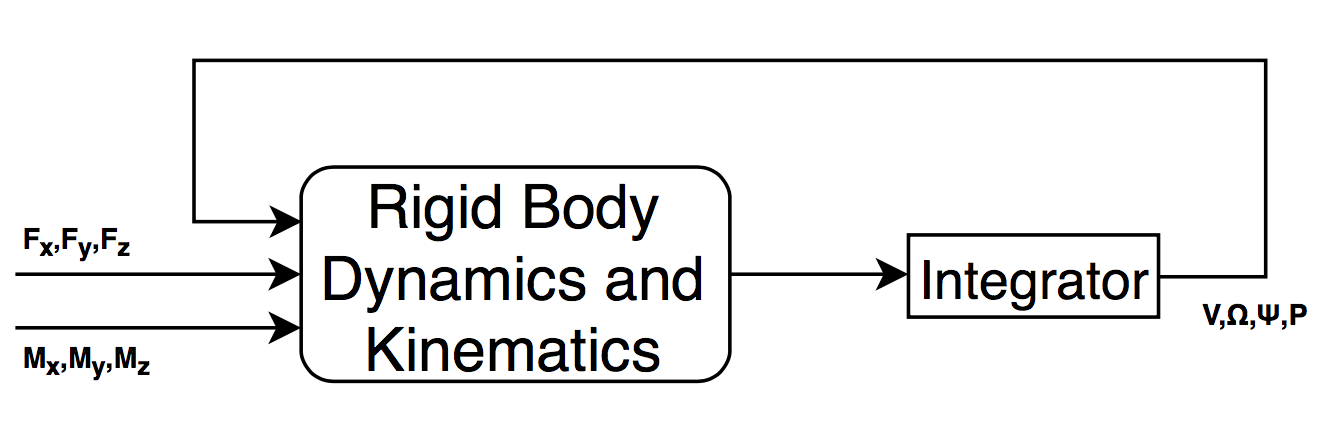
\includegraphics[width=0.8\textwidth]{images/blockdiagram.png}
	\caption{Dynamics and Kinematics Block Diagram.}
	\label{dk}
\end{figure}

\section{Quaternions and Euler angles}
In Section \ref{2.1}, we have explained how the position of the quadcopter is expressed in the inertial frame and how the  velocity of the quadcopter is express in the body-fixed frame. Therefore, we need to be able to find a relationship between the two, so that we can move from one to the other.

Euler angles have to be applied as a sequence of rotations. This report will use the \textit{roll, pitch, yaw} convention. Therefore, the roll rotation will be $R(\phi)^{T}$, the pitch rotation will be $R(\theta)^{T}$ and the yaw rotation will be $R(\psi)^{T}$. Equation \ref{rollpitchyaweq} describe the quadcopter's orientation relative to the inertial frame in matrix form:

\begin{equation}
\label{rollpitchyaweq}
\begin{aligned}
 	R(\phi)^{T}=\begin{bmatrix}
 	1 & 0 & 0 \\
 	0 & cos\phi & sin\phi \\
 	0 & -sin\phi & cos\phi \\
 	\end{bmatrix}\\     R(\theta)^{T}=\begin{bmatrix}
 	cos\theta & 0 & -sin\theta \\
 	0 & 1 & 0 \\
 	sin\theta & 0 & cos\theta \\
 	\end{bmatrix}\\     R(\psi)^{T}=\begin{bmatrix}
 	cos\psi & sin\psi & 0 \\
 	-sin\psi & cos\psi & 0 \\
 	0 & 0 & 1 \\
 	\end{bmatrix}
\end{aligned}
\end{equation}
 
Merging the three rotations as: 

\begin{equation}
\label{S1}	
 	S=R(\phi)^{T}R(\theta)^{T}R(\psi)^{T}
\end{equation}
 
gives the rotation matrix - \textit{S}, which expresses a vector from the inertial frame to the body-fixed frame: 
 
\begin{equation}
\label{S2}
 S=\begin{bmatrix}
 	cos\theta cos\psi & cos\theta sin\psi & -sin\theta \\
 	cos\psi sin\phi sin\theta-cos\phi sin\psi & sin\psi sin\theta sin\phi+cos\phi cos\psi & cos\theta sin\phi \\
 	cos\psi cos\phi sin\theta & cos\phi sin\theta sin\psi-cos\psi sin\phi & cos\theta cos\phi \\
\end{bmatrix}
\end{equation}
 	 
We can notice that if we were to have $\theta=\frac{\Pi}{2}$, the rotation matrix brings out a singularity by turning into:

\begin{equation}
\label{S3}
 S=\begin{bmatrix}
 	0 & 0 & -1 \\
 	sin(\phi-\psi) & cos(\phi-\psi) & 0 \\
 	cos(\phi-\psi) & -sin(\phi-\psi) & 0 \\
\end{bmatrix}
\end{equation}
 	 
As a result, one degree of freedom in the three dimensional space is lost. In addition, a change in either $\phi$ or $\psi$ will now have the same effect, which causes confusion. In order to be able to avoid this problem, a quaternion-based method can be applied instead. 

A quaternion can be expressed as $q=[q_{0}, q_{1}, q_{2}, q_{3}]^{T}$, which yields:

\begin{equation}
\label{S4}
 q=\begin{bmatrix}
 	cos(\phi/2) cos(\theta/2) cos(\psi/2) + sin(\phi/2) sin(\theta/2) sin(\psi/2) \\
 	sin(\phi/2) cos(\theta/2) cos(\psi/2) - cos(\phi/2) sin(\theta/2) sin(\psi/2) \\
 	cos(\phi/2) sin(\theta/2) cos(\psi/2) + sin(\phi/2) cos(\theta/2) sin(\psi/2) \\
 	cos(\phi/2) cos(\theta/2) sin(\psi/2) - sin(\phi/2) sin(\theta/2) cos(\psi/2)
\end{bmatrix}
\end{equation}
 	 
The quaternion and Euler angles are equivalent in terms of attitude, therefore we can convert from one representation to the other. The rotation matrix can be then rewritten as:

\begin{equation}
\label{S5}
 S_{q}=\begin{bmatrix}
 	1-2(q_{2}^{2}+q_{3}^{2}) & 2(q_{1}q_{2}+q_{3}q_{0}) & 2(q_{1}q_{3}-q_{2}q_{0}) \\
 	2(q_{1}q_{2}-q_{3}q_{0}) & 1-2(q_{1}^{2}+q_{3}^{2}) & 2(q_{2}q_{3}+q_{1}q_{0})  \\
 	2(q_{1}q_{3}+q_{2}q_{0}) & 2(q_{2}q_{3}-q_{1}q_{0}) & 1-2(q_{1}^{2}+q_{2}^{2}) \\
\end{bmatrix}
\end{equation}

\section{Quaternions Representation}
Knowing the position of the quadcopter relative to the inertial frame, the linear velocity in the body frame and the rotation matrix, a relationship between the three can be identified as:

\begin{equation}
\label{S6}
 \begin{bmatrix}
 	\dot{X} \\
 	\dot{Y} \\
 	\dot{Z} \\
 	\end{bmatrix}=S_{q}^{T}\begin{bmatrix}
 	U \\
 	V \\
 	W \\
 	\end{bmatrix}
 	 \end{equation}
 	 
The quadcopter's attitude can be written using the angular velocities vector $\Omega^{B}=[P, Q, R]^{T}$:

\begin{equation}
\label{S7}
 \begin{bmatrix}
 	\dot{q_{0}} \\
 	\dot{q_{1}}\\
 	\dot{q_{2}} \\
 	\dot{q_{3}} \\
 	\end{bmatrix}=\frac{1}{2}\begin{bmatrix}
 	0 & -P & -Q & -R \\
 	P & 0 & R & -Q \\
 	Q & -R & 0 & P \\
 	R & Q & -P & 0 \\
 	\end{bmatrix}\begin{bmatrix}
 	q_{0} \\
 	q_{1}\\
 	q_{2} \\
 	q_{3} \\
\end{bmatrix}
\end{equation}

Because we chose to neglect all other forces acting on the quadcopter except of the propeller thrust and gravity, we can further express the forces produced by the propellers along the $u_{z}$ axis as $[F_{1}, F_{2}, F_{3}, F_{4}]^{T}$. Therefore, the force in the body-fixed frame can be written as $F^{B}=[F_{x}, F_{y}, F_{z}]^{T}=[0, 0, -\sum\limits_{i=1}^4 F_{i}]^{T}$. Each force produces a moment around the axes of the quadcopter and as a result the moment in the body-fixed frame can be expressed as: $M^{B}=[M_{x}, M_{y}, M_{z}]^{T}$. These moments are explained in more detail in Section \ref{propModel}.

The dynamics of the quadcopter in regards to the rotations are given by $I\dot{\Omega}=-\Omega\times I \Omega+M_{B}$, which yields:

\begin{equation}
\label{S8}
 \begin{bmatrix}
 	\dot{P} \\
 	\dot{Q} \\
 	\dot{R} \\
 	\end{bmatrix}=\begin{bmatrix}
 	\frac{M_{x}}{I_{x}}  \\
 	\frac{M_{y}}{I_{y}}  \\
 	\frac{M_{z}}{I_{z}}  \\
 	\end{bmatrix}-\begin{bmatrix}
 	\frac{(I_{z}-I_{y})QR}{I_{x}} \\
 	\frac{(I_{x}-I_{z})QR}{I_{y}} \\
 	\frac{(I_{y}-I_{x})QR}{I_{z}} \\
\end{bmatrix}
\end{equation}
 	 
where the inertia matrix is:
\begin{equation}
\begin{bmatrix}
 	I_x & 0 & 0 \\
 	0 & I_y & 0 \\
 	0 & 0 & I_z \\
\end{bmatrix}
\end{equation}

Finally, by applying Newton's second law, we obtain $m a^{B}=F^{B}+m S_{q} g^{I} - \Omega \times V^{B}$, where $a^{B}=\dot{V}^{B}=[\dot{U}, \dot{V}, \dot{W}]^{T}$ is the acceleration vector and $g^{I}=[0, 0, g_{0}]^{T}$ is the gravity vector with $g=9.81m/s^{2}$.

Therefore:

\begin{equation}
\label{S10}
 \begin{bmatrix}
 	\dot{U} \\
 	\dot{V} \\
 	\dot{W} \\
 	\end{bmatrix}= \frac{1}{m}\begin{bmatrix}
 	F_{x}  \\
 	F_{y}   \\
 	F_{z}   \\
 	\end{bmatrix} + g_{0}\begin{bmatrix}
 	2(q_{1}q_{3}-q_{2}q_{0}) \\
 	2(q_{2}q_{3}+q_{1}q_{0}) \\
 	1-2(q_{1}^{2}+q_{2}^{2}) \\
 	\end{bmatrix} - \begin{bmatrix}
 	QW -RV \\
 	RU - PW \\
 	PV - QU \\
\end{bmatrix}
\end{equation}

\section{Euler Representation}
In order to make the Euler angle rates correspond to the angular velocity vector, we can write:

\begin{equation}
\label{S11}
 \begin{bmatrix}
 	P \\
 	Q \\
 	R \\
 	\end{bmatrix}=R(\phi)^{T}R(\theta)^{T}R(\psi)^{T}\begin{bmatrix}
 	0  \\
 	0  \\
 	\dot{\psi}  \\
 	\end{bmatrix}+R(\phi)^{T}R(\theta)^{T}\begin{bmatrix}
 	0  \\
 	\dot{\theta}  \\
 	0  \\
 	\end{bmatrix}+R(\phi)^{T}\begin{bmatrix}
 	\dot{\phi}  \\
 	0  \\
 	0  \\
\end{bmatrix}
\end{equation}

Solving for Euler angles rates finally gives:

\begin{equation}
\label{S10}
 \begin{bmatrix}
 	\dot{\phi} \\
 	\dot{\theta} \\
 	\dot{\psi} \\
 	\end{bmatrix}=\begin{bmatrix}
 	1 & tan\theta sin\phi & tan\theta cos\phi \\
 	0 & cos\phi & -sin\phi  \\
 	0 & sin\phi / cos\theta & cos\phi / cos\theta  \\
 	\end{bmatrix}\begin{bmatrix}
 	P \\
 	Q \\
 	R \\
\end{bmatrix}
\end{equation}